\chapter{E2E Test Framework}
\label{chap:e2e-test-framework}

\section{Automated E2E Testing}
\label{sec:automated-e2e-testing}

\subsection{Manual vs Automatic E2E Testing}
\label{sec:manual-vs-automatic-e2e-testing}

\subsection{Technologies Used}
\label{sec:technologies-used}

\section{Test Framework Components}
\label{sec:test-framework-components}

\subsection{Feature Definition as Requirements}
\label{subsec:feautre-definition-as-requirements}

Feature files can be seen as an entry point to cucumber test cases \cite{featurefile1}. Each of the feature file should be written to test a single feature of the application or a particular area of feature \cite{featurefile2}. Since we were writing E2E tests for the payment feature, we created \texttt{buycredits.feature} file for testing this aspect. Consider \textbf{Listing \ref{lst:buycredits-feature-file}}:\\

\begin{listing}[H]
\begin{minted}[xleftmargin=\parindent, linenos, breaklines, breakanywhere, bgcolor=lightgray, fontsize=\small]{cucumber}
@dev @experiment
Feature: Buying Credit feature
  As a user of Synote
  I should be able to successfully buy credits when logged in

  Scenario: Access buy credits page when logged in
    Given I click the "Profile" button on "SideMenu" page
    Given I click the "BuyCredit" button on "Profile" page
    Then I should be on "BuyCredits" page

  Scenario: Buy credit with empty card number
    Given I click the "Profile" button on "SideMenu" page
    Given I click the "BuyCredit" button on "Profile" page
    Given I Correctly type in my details but "" for "number"
    Then Submit button should be disabled
# code omitted
\end{minted}
\captionof{listing}{Section of \texttt{buycredits.feature} file}
\label{lst:buycredits-feature-file}
\end{listing}

The section in \textbf{Listing \ref{lst:buycredits-feature-file}} is written in a language called \texttt{Gherkin}. \texttt{Gherkin} makes use of Business Readable Domain Specific Language (BRDSL) which allows us to write the test cases at a business level without getting into implementation details.

Our client required us to document the requirements/specification for the new payment feature. Most of Synote's team are developers and since the feature file used \texttt{Gherkin}, it was readable on a business level and could act as automation test script \cite{featurefile1}. Hence, we recommended using the feature files themselves as the requirements documentation.\\

Each of the feature file should be defined with \texttt{Feature} keyword which consists of a name  (see \textbf{Listing \ref{lst:buycredits-feature-file}} line  2) and brief description  (see \textbf{Listing \ref{lst:buycredits-feature-file}} line  3-4). Each of the test cases are defined with \texttt{Scenario} keyword followed by a brief description of that test (see \textbf{Listing \ref{lst:buycredits-feature-file}} line  6 and 11). Each scenario should \cite{featurefile3}:
\begin{itemize}
\item Describe event taking place
\item Describe expected result
\end{itemize}

We use \texttt{Steps} to achieved this. Consider the \texttt{Access buy credits page when logged in} scenario in \textbf{Listing \ref{lst:buycredits-feature-file}}. We use keywords such as \texttt{Given} (line 7 and 8), \texttt{Then} (line 9) for writing readable test cases. Consider \textbf{Table \ref{tab:steps-keywords}} which define \texttt{Step} keywords \cite{featurefile1}

\begin{center}
%Column widths dependent on page width/margins
\begin{tabular}{ |p{2cm}|p{7cm}| }

 \hline
 	Keyword &
 	Description\\
 \hline
 	Given & Describes test pre-condition\\
 \hline
 	And & Defines additional test conditions\\
 \hline
 	Then & Defines expectations of test \\
 \hline

\end{tabular}
\captionof{table}{\texttt{Step keywords}}
\label{tab:steps-keywords}
\end{center}

\subsection{Reusable Steps Definition}
\label{subsec:reusable-steps-definition}

Cucumber is not able to execute the scenarios as they are. Instead, we have to write \texttt{step} definitions. Step definitions use regular expression to map the \texttt{Gherkin steps} to actions which will drive system interactions \cite{stepfile1}. Each of the \texttt{steps} written for scenarios in the \texttt{feature} file should have a \texttt{step} definition declared in its corresponding \texttt{step} file.\\ A \texttt{step} file should only contain definitions for \texttt{steps} used in corresponding \texttt{feature} file. Consider \textbf{Listing \ref{lst:buycredits-step-file}}:\\

\begin{listing}[H]
\begin{minted}[xleftmargin=\parindent, linenos, breaklines, breakanywhere, bgcolor=lightgray, fontsize=\small]{js}
@dev @experiment
//code omitted
this.Given(/^I click the "([^"]*)" button on "([^"]*)" page$/,
  function (buttonName, pageName) {
    return this.Support.clickButton(buttonName, pageName);
});

this.Given(/^I should be on "([^"]*)" page$/, function (pageName) {
  return this.Support.waitUntil
      (this.Support.urlChanged(this.Support.getPageUrl(pageName))
    , 2000)();
});
//code omitted
\end{minted}
\captionof{listing}{Section of \texttt{buycredits.steps.js} file}
\label{lst:buycredits-step-file}
\end{listing}

In our case, all the \texttt{steps} written in \texttt{buycredits.feature} file are defined in the \texttt{buycredits.steps.js} file. Each step should have a unique definition else an \texttt{ambiguous match} exception will be thrown. \textbf{Listing \ref{lst:buycredits-step-file}} contains the step definitions for \texttt{Access buy credits page when logged in} scenario in \textbf{Listing \ref{lst:buycredits-feature-file}}. Inside the step definitions, we write javascript code to handle the interaction logic e.g. 1st definition in \textbf{Listing \ref{lst:buycredits-step-file}} (line 3) handles clicking of button provided  \texttt{buttonName and pageName} parameters and 2nd definition (line 7) handles checking we are on a page with certain URL provided  \texttt{pageName} parameter. Nearly all of out step definitions take parameters instead of hard-coding them. This way, we can satisfy the \texttt{DRY} principle by reusing generic step definitions, making both  \texttt{feature} and  \texttt{step} files easily maintainable and readable in the long run.

\subsection{Reusable Support Functions}
\label{subsec:reusable-support-functions}

In order to have generic \texttt{step} definitions (e.g. see \textbf{Listing \ref{lst:buycredits-step-file}} line 3 and 7), we needed to write common generic methods which will drive interactions with the system. We place such functions in the \texttt{support.js} file. As a rule of thumb, we identified generic methods to go in the \texttt{support.js} file by checking if were were repeating any code/logic in the \texttt{bycredits.steps.js} file. Currently, our frame work uses the \texttt{support.js} file for:

\begin{itemize}
\item Clicking
\item Filling inputs
\item Navigating
\item Data retrieval
\end{itemize}

\begin{listing}[H]
\begin{minted}[xleftmargin=\parindent, linenos, breaklines, breakanywhere, bgcolor=lightgray, fontsize=\small]{js}
@dev @experiment
//code omitted
function loadPageOnSupport(pageName) {
  if (!support[pageName]) {
    support[pageName] = require
      ('../pages/' + pageName.toLowerCase() + '.page.js');
  }
}
//code omitted
fillInputOnPage: function (pageName, textBox, text) {
  loadPageOnSupport(pageName);
  if (this[pageName] && this[pageName][textBox + 'Input']) {
    var _textBox = this[pageName][textBox + 'Input'];
    return _textBox.sendKeys(text);
  }
}
//code omitted
\end{minted}
\captionof{listing}{Section of \texttt{support.js} file}
\label{lst:support-file-methods}
\end{listing}

Consider \textbf{Listing \ref{lst:support-file-methods}}. The \texttt{fillInputOnPage} is a common generic method i.e. it can be used to fill any input field on any page, hence its placement in the \texttt{support.js} file. The \texttt{loadPageOnSupport} method helps \texttt{support.js} file to be generic in applying its methods in different contexts by dynamically requiring desired pages objects. Main advantage of \texttt{support.js} is that testers will never have to rewrite any code they have already written, satisfying the \texttt{DRY} principle.

\subsection{Pre and Post Hooks}
\label{subsec:pre-and-post-hooks}

\subsection{Page Objects}
\label{subsec:page-objects}
There are few key interactions which are very common throughout the application e.g. clicking buttons, filling in inputs, navigating to pages etc. It seemed tedious and time consuming to actually write separate methods for these interactions on different pages. We came to the conclusion that the interactions themselves should be generic enough so they can be applied to any page. The pages of application differed in the elements and components they had. Hence, we have definitions of \texttt{Page Object Models} which is composed of elements a page has.

\begin{minipage}{.48\textwidth}
\begin{listing}[H]
\begin{minted}[xleftmargin=\parindent, linenos, breaklines, breakanywhere, bgcolor=lightgray, fontsize=\small]{js}
{ // buyCredits.page.js snippet
Title : "BuyCredits",
Url : browser.deployment.hostUrl + 'buycredit',

billing_nameInput : element
  (by.model('billingName')),

numberInput : element
  (by.model('cardNumber')),

cvcInput : element
  (by.model('cardCVC')),

exp_monthInput : element
  (by.model('expMonth')),

exp_yearInput : element
  (by.model('expYear')),

PaySavedRadioButton : element
  (by.id('pay-saved-radio')),
//code omitted
}
\end{minted}
\captionof{listing}{Section of \texttt{buycredits.page.js} file}
\label{lst:buycredits-page-code}
\end{listing}
\vspace{0.1cm}
\end{minipage}%
\begin{minipage}{.49\textwidth}
  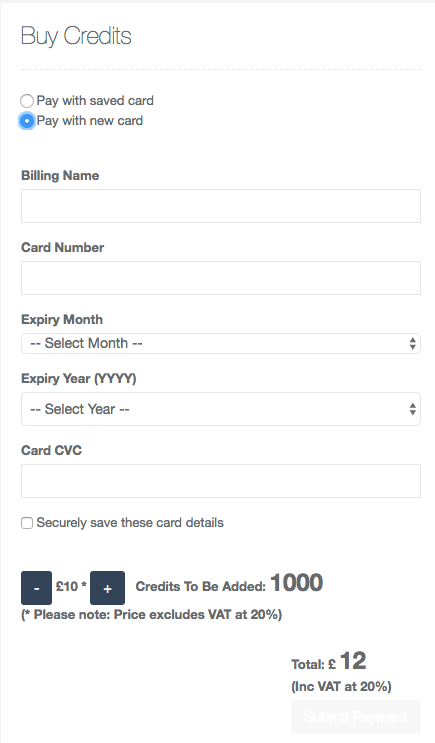
\includegraphics[width=\textwidth]{screenshot-payment-form.png}
  \captionof{figure}{Payment Form}
 	\label{fig:paymentform-screenshot}
\end{minipage}

Here we have the \texttt{buycredits.html} page (\textbf{Figure \ref{fig:paymentform-screenshot}}) and it's corresponding \texttt{buycreditspage.js} \textit{page object file} (\textbf{Listing \ref{lst:buycredits-page-code}}) which is basically a one to one mapping from the html page components. Page object files also house methods to interact with elements (defined in the same \textit{page object model}) which are only applicable to the particular page in question e.g. \texttt{buycreditspage.js} has a method called \texttt{fillDefaultCardDetails} which fills in the payment form fields and is only applicable to \texttt{buycredits.html} page. The main advantages of implementing page objects were reduced code duplication and easy maintainability i.e.  if any of the UI element of the application was changed, we only have to modify them in the page object file instead of fixing them in each \texttt{step} which used that UI element \cite{semaphore}. Another advantage is that it structures the framework, improving readability.

\subsection{Deployment Definition}
\label{subsec:deployment-definition}
One of the requirements of our client was that our framework should be capable of running the E2E test suite against different deployments of Synote application. The main concern we had here was that tests which worked on one deployment may not work on another deployment because each deployments of Synote is uses different parameters. For example host url of \texttt{development} deployment is \texttt{http://localhost:9000/\#/} and for  \texttt{experiment} deployment, it is \texttt{https://experiment.synote.com/\#/}. Same with other parameters such as cards e.g. \texttt{development} should use test card whereas live deployments such as \texttt{experiment} should use live cards. It can be very time consuming to manually enter all this data when you want to test a deployment. To overcome this problem, we created \texttt{deployment.js} file which can be used to easily define different deployments of Synote application.

\begin{listing}[H]
\begin{minted}[xleftmargin=\parindent, linenos, breaklines, breakanywhere, bgcolor=lightgray, fontsize=\small]{js}
//code omitted
deployment_name : { // e.g. experiment
  hostUrl : 'deployment_url', // e.g. https://experiment.synote.com
  apiEndpoint : 'backend_rest_api_url',
  defaultUser: {
    password : 'password',
    role: 'test_user_role'
  },
  defaultCard: {
    // test card for dev, real card for staging etc.
  }
}
//code omitted
\end{minted}
\captionof{listing}{Section of \texttt{deployment.js} file}
\label{lst:deployment-file}
\end{listing}

Consider \textbf{Listing \ref{lst:deployment-file}}. Here you can see that each deployment of Synote is defined by different parameters. This way, you only have to define deployment specific data once for running the tests.

\begin{listing}[H]
\begin{minted}[xleftmargin=\parindent, linenos, breaklines, breakanywhere, bgcolor=lightgray, fontsize=\small]{bash}
	conf.js --params.env dev --cucumberOpts.tgs=@deployment_name
\end{minted}
\captionof{listing}{Running the E2E Tests}
\label{lst:specifying-deployment-test-run}
\end{listing}

When running the E2E tests, we simply need to pass the name of object which represents the deployment we want to test against. For example: consider \textbf{Listing \ref{lst:specifying-deployment-test-run}}, here we pass in \texttt{dev} as a parameter so the framework will execute tests on \texttt{development} deployment with data defined in \texttt{dev} object.  To overcome the issues with some tests only being suitable for certain deployments, we used \texttt{cucumber tags} which can be placed on \texttt{feature} keyword of \texttt{feature} files or on desired \texttt{scenarios}. For example, in \textbf{Listing \ref{lst:buycredits-feature-file}} we place \texttt{dev} and \texttt{experiment} keywords on the \texttt{feature} keyword so all the test \texttt{scenarios} will run for both of these deployments. The desired test suite to be executed has to be specified as a parameter when executing the tests (see \textbf{Listing \ref{lst:specifying-deployment-test-run}}).

 \subsection{Example Test Case}
\label{subsec:example-test-case}

When testing a feature of the application, we initially start with a requirement which will later form the description of the \texttt{feature file}. For example, say we want to test the \texttt{payment feature} and our requirement is \texttt{As a user of Synote I should be able to successfully buy credits when logged in}. First we will need to create a feature file as in \textbf{Listing \ref{lst:example-feature-file}}.

\begin{listing}[H]
\begin{minted}[xleftmargin=\parindent, linenos, breaklines, breakanywhere, bgcolor=lightgray, fontsize=\small]{cucumber}
Feature: Buying Credit feature
  As a user of Synote
  I should be able to successfully buy credits when logged in
\end{minted}
\captionof{listing}{Example feature for payment feature}
\label{lst:example-feature-file}
\end{listing}

In \textbf{Listing \ref{lst:example-feature-file}} we use the \texttt{feature} keyword to title the feature under test i.e. \texttt{payment feature} and describe it via the requirement. The requirement is then broken down into sub-requirements which will together satisfy the main requirement. The sub-requirements are written as \texttt{scenarios}. For example, say our sub-requirement was \texttt{Buy credit with valid card details}, then its corresponding \texttt{scenario} will look like:

\begin{listing}[H]
\begin{minted}[xleftmargin=\parindent, linenos, breaklines, breakanywhere, bgcolor=lightgray, fontsize=\small]{cucumber}
# code omitted
Scenario: Buy credit with valid card details
  Given I click the "Profile" button on "SideMenu" page
  Given I click the "BuyCredit" button on "Profile" page
  Given I Correctly type in my details
  And I click the "SubmitPayment" button on "BuyCredits" page
  Then I should be on "CreditsHistory" page
\end{minted}
\captionof{listing}{Example \texttt{Feature} File}
\label{lst:example-feature-file-scenario}
\end{listing}

In \textbf{Listing \ref{lst:example-feature-file-scenario}}, we have labelled the \texttt{scenario} with the sub-requirement definition itself and wrote \texttt{steps} in \texttt{Gherkin} for testing it. If any of the \texttt{steps} take parameter, we specify them with quotes.\\

Next we need to is create a \texttt{steps} file where step definitions for the 5 steps in \textbf{Listing \ref{lst:example-feature-file-scenario}} will be written. Consider \textbf{Listing \ref{lst:example-steps-file}}.

\begin{listing}[H]
\begin{minted}[xleftmargin=\parindent, linenos, breaklines, breakanywhere, bgcolor=lightgray, fontsize=\small]{js}
module.exports = function () {
  this.Given(/^I click the "([^"]*)" button on "([^"]*)" page$/,
    function (buttonName, pageName) {
  });
  this.Given(/^I Correctly type in my details$/, {timeout: 60*1000},
    function () {
  });
  this.Given(/^I should be on "([^"]*)" page$/,
    function (pageName) {
      //return this.Support.waitUntil
      //  (this.Support.urlChanged(this.Support.getPageUrl(pageName))
      // , 2000)();
  });
}
\end{minted}
\captionof{listing}{Example \texttt{Steps File}}
\label{lst:example-steps-file}
\end{listing}

In \textbf{Listing \ref{lst:example-steps-file}} we define the \texttt{steps} written in \textbf{Listing \ref{lst:example-feature-file-scenario}} using reqular expressions. The \texttt{scenario} in \textbf{Listing \ref{lst:example-feature-file-scenario}} will be interacting with the payment form (\textbf{See Figure \ref{fig:paymentform-screenshot}}) and so we need to create a \texttt{page object} file for it as defined in  \textbf{Section \ref{subsec:page-objects}}.

\begin{listing}[H]
\begin{minted}[xleftmargin=\parindent, linenos, breaklines, breakanywhere, bgcolor=lightgray, fontsize=\small]{js}
var buyCreditsPage = {
  Title : "BuyCredits",
  Url : browser.deployment.hostUrl + 'buycredit',
  billing_nameInput : element(by.model('billingName')),
  numberInput : element(by.model('cardNumber')),
  cvcInput : element(by.model('cardCVC'))
  //code omitted
}
\end{minted}
\captionof{listing}{Example \texttt{Page Object} File}
\label{lst:example-page-file}
\end{listing}

In \textbf{Listing \ref{lst:example-page-file}}, we created a one to one mapping of all the elements of the payment form. Next step is to actually write interaction code to complete the step definitions in \textbf{Listing \ref{lst:example-steps-file}} with the help of page object.\\

Consider the 1st \texttt{step} definition in \textbf{Listing \ref{lst:example-steps-file}}. This can be grouped as a generic \texttt{step} since it can be applicable to many elements on different pages. Therefore we should create a generic method in \texttt{support.js} file for this interaction as mentioned in  \textbf{Section \ref{subsec:reusable-support-functions}}. Consider  \textbf{Listing \ref{lst:example-support-func}}

\begin{listing}[H]
\begin{minted}[xleftmargin=\parindent, linenos, breaklines, breakanywhere, bgcolor=lightgray, fontsize=\small]{js}
clickButton: function (buttonName, pageName) {
  loadPageOnSupport(pageName);
  var button = support.getButton(buttonName, pageName);
  return button.click();
},
\end{minted}
\captionof{listing}{Example Support Function for clicking}
\label{lst:example-support-func}
\end{listing}

\textbf{Listing \ref{lst:example-support-func}} shows section of the \texttt{support} file with the generic method to handle clicking. See \textbf{Listing \ref{lst:example-step-def-click-completed}} to see usage of this function in the step definition.

\begin{listing}[H]
\begin{minted}[xleftmargin=\parindent, linenos, breaklines, breakanywhere, bgcolor=lightgray, fontsize=\small]{js}
//code omitted
this.Given(/^I click the "([^"]*)" button on "([^"]*)" page$/,
  function (buttonName, pageName) {
    return this.Support.clickButton(buttonName, pageName);
});
//code omitted
\end{minted}
\captionof{listing}{Completed Step Definition For Clicking Buttons}
\label{lst:example-step-def-click-completed}
\end{listing}

Now consider the 2nd \texttt{step} definition in \textbf{Listing \ref{lst:example-steps-file}}. This \texttt{step} is specific to the payment form only. Hence this interaction should be handled in the \texttt{page object} file for payment form.

\begin{listing}[H]
\begin{minted}[xleftmargin=\parindent, linenos, breaklines, breakanywhere, bgcolor=lightgray, fontsize=\small]{js}
//code omitted
fillInputsOnPage : function (pageName, fieldValMap){
  loadPageOnSupport(pageName);
  if (support[pageName]) {
    var promises = [];
    // enter the exception fields
    _.forOwn(fieldValMap, function (val, field) {
      if (field && val) {
        promises.push(support.fillInputOnPage(pageName, field, val));
      }
    });
    return Promise.all(promises);
  }
}
//code omitted
\end{minted}
\captionof{listing}{Payment Form Page Specific Method for Filling in Fields}
\label{lst:example-page-specific-method}
\end{listing}

\textbf{Listing \ref{lst:example-page-specific-method}} shows section of the \texttt{page} file with implementation of method to fill inputs of payment form. See \textbf{Listing \ref{lst:example-step-def-fillin-completed}} to see usage of this function in the step definition.

\begin{listing}[H]
\begin{minted}[xleftmargin=\parindent, linenos, breaklines, breakanywhere, bgcolor=lightgray, fontsize=\small]{js}
//code omitted
this.Given(/^I Correctly type in my details$/, {timeout: 60*1000},
  function () {
    return this.BuyCreditsPage.fillDefaultCardDetails();
});
//code omitted
\end{minted}
\captionof{listing}{Completed Step Definition For Filling in Payment Form}
\label{lst:example-step-def-fillin-completed}
\end{listing}

Finally, Consider the 3st \texttt{step} definition in \textbf{Listing \ref{lst:example-steps-file}}. This can also be grouped as a generic \texttt{step} since it is applicable to different pages. Here we need to create the following methods in \texttt{support} file for:

\begin{itemize}
\item Waiting a certain time for page to load
\item Checking current URL matches passed in URL
\end{itemize}

\begin{listing}[H]
\begin{minted}[xleftmargin=\parindent, linenos, breaklines, breakanywhere, bgcolor=lightgray, fontsize=\small]{js}
//code omitted
waitUntil : function (action, time) {
  return function () {
    return browser.wait(action, time);
  }
},

urlChanged : function(url) {
  return function () {
    return browser.getCurrentUrl().then(function(actualUrl) {
      return actualUrl === url;
    });
  };
},
//code omitted
\end{minted}
\captionof{listing}{Example Support Function For Checking Page URL}
\label{lst:example-support-func2}
\end{listing}

\textbf{Listing \ref{lst:example-support-func2}} shows implementation generic methods required to complete the final step definition. See \textbf{Listing \ref{lst:example-step-def-url-check-completed}} to see usage of these function in the step definition.

\begin{listing}[H]
\begin{minted}[xleftmargin=\parindent, linenos, breaklines, breakanywhere, bgcolor=lightgray, fontsize=\small]{js}
//code omitted
this.Given(/^I should be on "([^"]*)" page$/, function (pageName) {
  return this.Support.waitUntil
      (this.Support.urlChanged(this.Support.getPageUrl(pageName))
    , 2000)();
});
//code omitted
\end{minted}
\captionof{listing}{Completed Step Definition For Verifying Current URL}
\label{lst:example-step-def-url-check-completed}
\end{listing}

\subsection{Reporting}
\label{subsec:reporting}

\subsection{Assessment}
\label{subsec:assessment}

The framework's capabilities where thoroughly tested by Deepak, who wrote most of the test cases. Tom focused on the second iteration of the payment feature and was purposefully not involved in the initial prototyping of the testing framework. This enabled Tom to have an outside perspective of the framework to provide an assessment of its ease of use. Armed with the framework repository and a readme file, Tom set about writing a test for the latest payment feature functionality he had added.\\

Following the readme file, the first step is to install the dependencies. This was the first time the framework had been installed on a Windows machine and due to an installation of Visual Studio, an error occurred. After resolving this issue, the relevant steps were added to the readme and progress resumed. After browsing the existing files relevant to each section in the readme, it was apparent that nearly all the tools Tom needed existed already. Lines 1-3 \& 5 of \textbf{Listing \ref{lst:toms-first-test}} make use of existing step methods however, line 4 required an extension of the existing method in \textbf{Listing \ref{lst:buycredits-step-file}} to allow repeated clicks as shown in \textbf{Listing \ref{lst:additional-step-method}}.\\

\begin{listing}[H]
\begin{minted}[xleftmargin=\parindent, linenos, breaklines, breakanywhere, bgcolor=lightgray, fontsize=\small]{cucumber}
Scenario: Maximum purchase cost reached
  Given I click the "Profile" button on "SideMenu" page
  Given I click the "BuyCredit" button on "Profile" page
  Given I click the "IncrementCredit" button on "BuyCredits" page 59 times
  Then Increment credit button should be disabled
\end{minted}
\captionof{listing}{Tom's First Test}
\label{lst:toms-first-test}
\end{listing}

\begin{listing}[H]
\begin{minted}[xleftmargin=\parindent, linenos, breaklines, breakanywhere, bgcolor=lightgray, fontsize=\small]{js}
this.Given(/^I click the "([^"]*)" button on "([^"]*)" page (\d+) times$/,
  function (buttonName, pageName, times) {
    var promises = [];
    for(var i = 0; i < times; i++) {
      promises.push(this.Support.clickButton(buttonName, pageName));
    }
    return Promise.all(promises);
});
\end{minted}
\captionof{listing}{Additional Step Method}
\label{lst:additional-step-method}
\end{listing}

Again, referring to the readme file, Tom ran the test suite on his local development machine and watched as the test he had written passed first time. As this was local testing, the actions were executed in a browser window providing visual confirmation that the desired actions were performed. Thus, with no prior knowledge, Tom was able to use the framework to write and execute a successful E2E test.
